\section{Background}
\label{sec:background}

\begin{figure*}[t]
  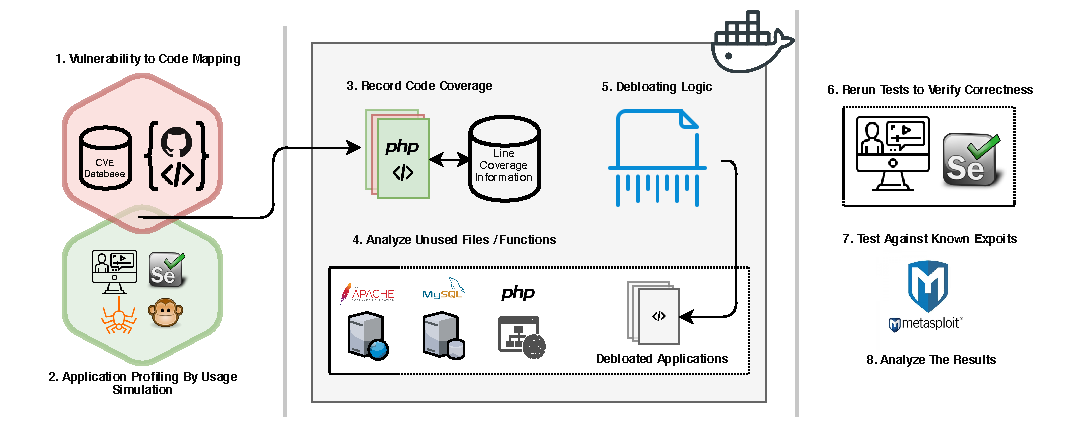
\includegraphics[width=\linewidth]{figures/lim/DebloatingPipeline.pdf}
  \vspace{-6ex}
  \caption{Overview of the architecture of our pipeline for debloating web applications and assessing the effects of different debloating strategies.}
  \vspace{-2ex}
  \label{fig:debloatingpipeline}
\end{figure*}

In this section, we briefly describe the effect of package managers on software
bloat and provide a motivating example for debloating web applications.


\subsection{Package managers and software bloat}
To ease the development of software, developers reuse third-party libraries,
external packages, and frameworks for their applications. This approach
enables developers to focus on their applications while relying on
proven and tested components. Statistics from popular package managers show
that reliance on external packages is a widely adopted practice across
many different languages. NPM, the registry hosting NodeJS packages,
reports more than 10 billion package downloads a
month~\cite{nodeDownloads}. Similarly, PyPI, the package manager for Python,
reports more than a billion a month~\cite{pypiDownloads}, while Packagist, the main repository for
Composer package manager for PHP, reports the download of 500 million
packages each month~\cite{packagistDownloads}.

At the same time, it is doubtful that \emph{all} the code and features
obtained through these packages and frameworks are actually used by
the applications that rely on them. For the most part, when developers rely on
external dependencies, they include entire packages with no effective way of
disabling and/or removing the parts of these packages and frameworks that
their applications do not require.

\subsection{Motivating web-application debloating}

In this study, we look at the bloat of web applications and quantify how
debloating can provide concrete security benefits. Even
though debloating has been successfully applied in other contexts, we argue
that the
idiosyncrasies of the web platform (e.g., the ambient authority of cookies and
the client/server model which is standard for the web but atypical
for operating systems and compiled software) require a dedicated analysis
of the applicability of debloating for web applications.

%As detailed in Section~\ref{sec:related}, several works have been
%published in the debloating domain but none of them looked specifically
%at web applications, nor did they tackle the subject from a security
%perspective. Indeed, web applications are vulnerable to different classes
%of attacks like code execution, denial of service or authentication bypass.
%Understanding the impact of debloating requires its own in-depth analysis
%that cannot be derived from other types of applications. Since we focus on
%the business logic of web applications, we decided upon PHP as the language
%used for this study. It is one of the most widely used server-side language
%in the world~\cite{phpAdoption} and very popular websites like Facebook,
%Yahoo or Wikipedia have a large part of their codebase written in this
%language. A package manager called Composer handles external dependencies
%in PHP~\cite{composer} and it relies on packages hosted on the Packagist
%website~\cite{packagist}.



To understand how the bloat of a web application can lead to a critical
vulnerability, we use a recent vulnerability of the Symfony web
framework (CVE-2018-14773~\cite{symfonyVulnerability}) as a motivating
example. Specifically, the Symfony web framework supported a legacy IIS
header that could be abused to have Symfony return a different URL than the
one in the request header, allowing the bypassing of web application firewalls
and server-side access-control mechanisms. If this type of header
was never used by the server, debloating the application would have removed
support for it, which ultimately would have prevented anyone from exploiting
the vulnerability. Drupal, a popular PHP Content Management System (CMS), was also affected by
the same vulnerability since it uses libraries from the Symfony framework
to handle parts of its internal logic~\cite{drupalVulenrability}. Even
if Drupal developers were not responsible for the code that leads to the
vulnerability, their application could still be exploited since Symfony
was an external dependency. Even more interestingly, an analysis of the
official Symfony patch on GitHub~\cite{symfonyPatch}
reveals that the vulnerable lines were derived from yet another framework
called Zend~\cite{zendVulnerability}. This shows that the structure of web
applications can be very complex with code reuse originating from many
different sources. Even if developers take all possible precautions to
minimize vulnerabilities in their own code, flaws from external dependencies
can cascade and lead to a critical entry point for an attacker.

Overall, there are clear benefits that debloating could have on web
applications. Assuming that we are able to pinpoint all the code that is required
by the users of a given software deployment, all other code (including the
code containing vulnerabilities) can be removed from that deployment.
